\section{Finding Double Unlock Bugs}

\newpar A requirement of this project was that the user of the analyzer should be able to supply their own analyses. We decided to enable this by having the user define a lattice and transfer functions. These structures are then used by the analyzer in order to gain knowledge about input programs.

\newpar Due to the requirement of a user passing their own analyses to the framework and the fact that these analyses need to be loaded at runtime, Python was used for the implementation of our analyzer. Given the dynamic nature of the Python programming language, evaluating Python scripts dynamically at runtime is relatively easy and supported by the language. Using a compiled language, e.g. OCaml, turned out to be too unstable in practice given the static compiled nature of the language. Loading in arbitrary user code is to a great extent not supported in compiled languages and this dynamic loading of arbitrary modules is where a dynamic language shines. 

\newpar The user supplies our framework with a list of file names containing Python class definitions. The framework then dynamically loads these analyses which the user is expected to formulate as individual Python scripts. These scripts must implement and expose an \texttt{Analysis} class containing the components our framework implementation expects to be present in order to analyze. 

\newpar A disadvantage in using a dynamic language is the lack of type checks. Python supports type annotations, but these are generally completely ignored by the interpreter. The type annotations read more like comments in the source code than actual safety guarantees. This means that we have no way of enforcing that the analyses supplied by the user adhere to an interface or a class definition, and we can only provide examples for the user to follow when implementing their analysis. This is unfortunate, since the framework will simply throw an \texttt{Error} when attempting to evaluate the users' analyses. Using a compiled language would allow us to specify a signature for the analyses of the user to implement, guaranteeing that the analysis could be run without errors --- provided that the users' own implementations does not raise errors.

\newpar The framework is invoked with a list of filenames of analysis files. These files are implemented as very basic Python modules, which are then imported at runtime. An invocation of the two analyses \texttt{AnalysisA} and \texttt{AnalysisB} would require the user to provide the list of analyses as to the framework as \texttt{"AnalysisA:AnalysisB"}. This list of names is split on commas, and the framework then attempts to import these modules. 
User analyses are expected to be located in the \texttt{analyzers} subfolder of the framework implementation in a corresponding subfolder. Due to the way Python expects modules to be structured, a file named \texttt{\_\_init\_\_.py} needs to be co-located with the analysis implementation file. This is merely a practicality in the way the Python module system works. An illustration of the module structure can be seen in Fig. \ref{fig:modulestructure}.

\begin{figure}[H]
    \centering
    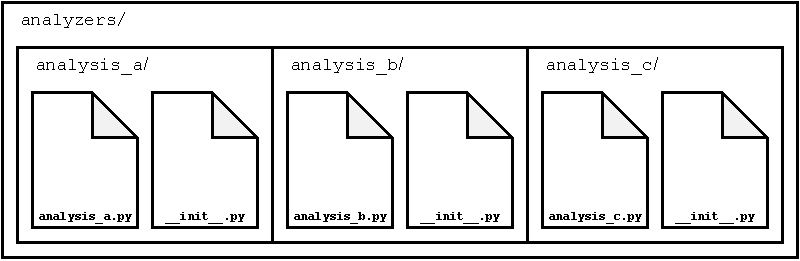
\includegraphics{implementation/figures/folderstructure}
    \caption{The folder structure for three analyses provided by the user.}
    \label{fig:modulestructure}
\end{figure}

\newpar An analysis provided by the user must expose an instance of an \texttt{Analysis} class. This class requires a list of transfer functions, variables and expressions to be provided for instantiation. The analyzer extracts this instance and applies the transfer functions for each provided \texttt{Analysis} to the input file. The result of applying an analysis results in a transformed input program, which is fed forward to the next provided \texttt{Analysis}. When no more analyses are present, the transformed input program is given as output to the user. An illustration of this can be seen in Fig. \ref{fig:programflow}.

\begin{figure}[H]
    \centering
    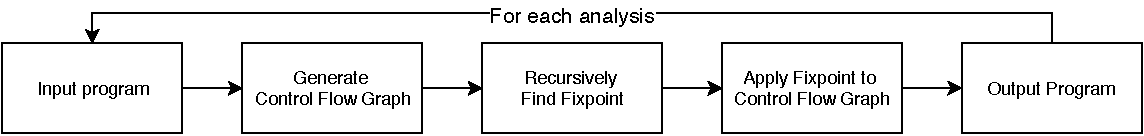
\includegraphics[width=\textwidth]{implementation/figures/programflow}
    \caption{The program flow for analyzing a program with multiple provided analyses.}
    \label{fig:programflow}
\end{figure}

